%iffalse
\let\negmedspace\undefined
\let\negthickspace\undefined
\documentclass[journal,12pt,onecolumn]{IEEEtran}
\usepackage{cite}
\usepackage{amsmath,amssymb,amsfonts,amsthm}
\usepackage{algorithmic}
\usepackage{graphicx}
\usepackage{textcomp}
\usepackage{xcolor}
\usepackage{txfonts}
\usepackage{listings}
\usepackage{enumitem}
\usepackage{mathtools}
\usepackage{gensymb}
\usepackage{comment}
\usepackage[breaklinks=true]{hyperref}
\usepackage{tkz-euclide} 
\usepackage{listings}
\usepackage{gvv}                                        
\def\inputGnumericTable{}                                 
\usepackage[latin1]{inputenc}                                
\usepackage{color}                                            
\usepackage{array}                                             
\usepackage{longtable}                                       
\usepackage{calc}                                             
\usepackage{multirow}                                         
\usepackage{hhline}                                           
\usepackage{ifthen}                                           
\usepackage{lscape}
\usepackage{multicol}

\newtheorem{theorem}{Theorem}[section]
\newtheorem{problem}{Problem}
\newtheorem{proposition}{Proposition}[section]
\newtheorem{lemma}{Lemma}[section]
\newtheorem{corollary}[theorem]{Corollary}
\newtheorem{example}{Example}[section]
\newtheorem{definition}[problem]{Definition}
\newcommand{\BEQA}{\begin{eqnarray}}
\newcommand{\EEQA}{\end{eqnarray}}
\newcommand{\define}{\stackrel{\triangle}{=}}
\theoremstyle{remark}
\newtheorem{rem}{Remark}
\begin{document}

\bibliographystyle{IEEEtran}
\vspace{3cm}

\title{NCERT - 6.5.14}
\author{EE224BTECH11044 - Muthyala koushik
}
\maketitle
\bigskip

\renewcommand{\thefigure}{\theenumi}
\renewcommand{\thetable}{\theenumi}
\textbf{\section{APPLICATION OF DERIVATIVES}}


\textbf{Question:} Find two positive numbers $x$ and $y$ such that $x + y = 60$ and $xy^3$ is maximized. \\

\solution

Let $z = xy^3$. From the equation $x + y = 60$, we can express $x$ as:  
\begin{align}
    x = 60 - y.
\end{align}

Substitute this into $z$:  
\begin{align}
    z &= xy^3 = (60 - y) \cdot y^3, \\
    z &= 60y^3 - y^4.
\end{align}

To maximize $z$, we take its derivative with respect to $y$ and set it equal to zero:  
\begin{align}
    \frac{dz}{dy} &= \frac{d}{dy}(60y^3 - y^4), \\
    \frac{dz}{dy} &= 180y^2 - 4y^3, \\
    \frac{dz}{dy} &= y^2(180 - 4y).
\end{align}

Setting $\frac{dz}{dy} = 0$:  
\begin{align}
    y^2(180 - 4y) = 0.
\end{align}

This gives two possibilities:  
\begin{itemize}
    \item $y^2 = 0 \implies y = 0$ (not valid as $y > 0$), and
    \item $180 - 4y = 0 \implies y = 45$.
\end{itemize}

Substituting $y = 45$ into $x + y = 60$:  
\begin{align}
    x = 60 - 45 \implies x = 15.
\end{align}

To confirm this is a maximum, calculate the second derivative of $z$:  
\begin{align}
    \frac{d^2z}{dy^2} &= \frac{d}{dy}(180y^2 - 4y^3), \\
    \frac{d^2z}{dy^2} &= 360y - 12y^2.
\end{align}

At $y = 45$:  
\begin{align}
    \frac{d^2z}{dy^2} &= 360(45) - 12(45^2), \\
    \frac{d^2z}{dy^2} &= 16200 - 24300, \\
    \frac{d^2z}{dy^2} &= -8100.
\end{align}

Since $\frac{d^2z}{dy^2} < 0$, the value of $z$ is maximized at $y = 45$. \\

\textbf{Final Answer:} The two numbers are $x = 15$ and $y = 45$.\\


\textbf{Solution by the method of Gradient Descent:}
Using the the method of gradient accent;
\begin{align}
	y_{n+1}=y_n+h*F^{'}(y_n)
\end{align}

from the equation above:
\begin{align}
	y_{n+1}=y_n+h*\brak{{y_n}^2\brak{180-4y_n}}
\end{align}
 
Choosing $y_0=20$, $\alpha=0.0001$, we get thave value of y as,
\begin{align}
	y=45
\end{align}

\begin{figure}[h]
	\centering
	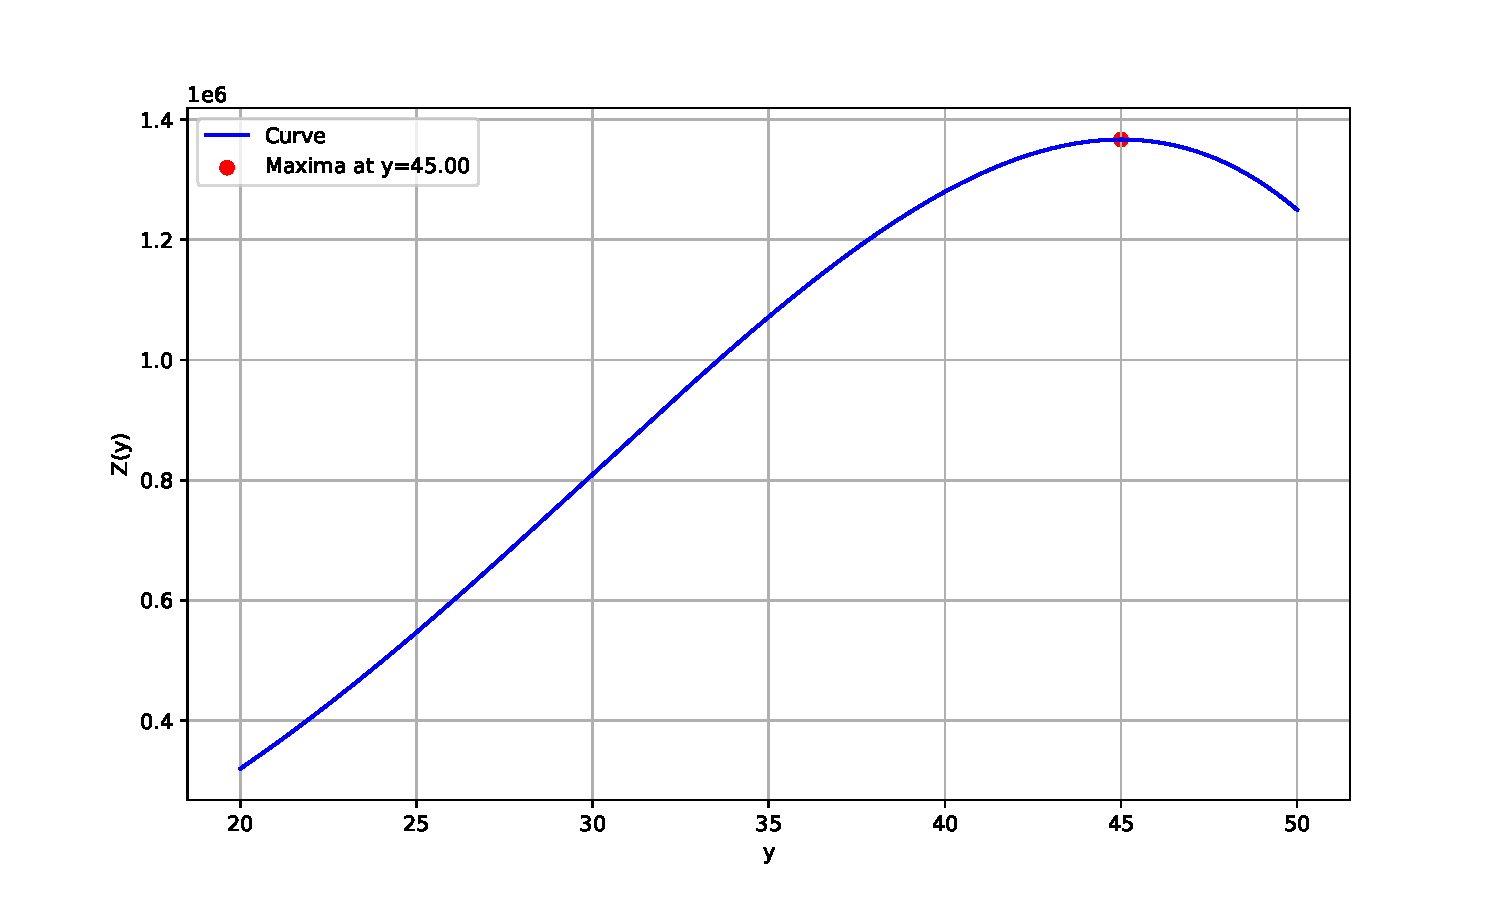
\includegraphics[width=\columnwidth]{figs/fig.pdf}
\end{figure}

\end{document}
